\chapter{Zahlenbereiche}
\section{Natürliche Zahlen}
Die natürlichen Zahlen 1, 2, 3, 4, \ldots ~sind die ältesten Zahlen, die sich aus dem Zählen von Gegenständen entwickelt haben.
Dabei nimmt man an, dass man immer weiterzählen kann.\\

\begin{defn}{Natürliche Zahlen}
	Die Menge der natürlichen Zahlen wird mit $\N$ bezeichnet.
	Man schreibt:
	\begin{align*} 
	 \N = \{ 1, 2, 3, 4, \ldots \}\, .
	\end{align*}
	Die Zahlen $1, 2, 3, 4, \ldots$ heissen \emph{Elemente} der Menge $\N$.
	Ist eine Zahl $n$ eine natürliche Zahl, so schreibt man: $n\in\N$\,.
\end{defn}

\vspace{.5cm}
\begin{wrapfigure}{r}{6cm}
	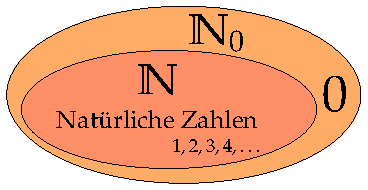
\includegraphics[width=\linewidth]{numberset-naturals-N0}
\end{wrapfigure}
Das Zeichen \glqq $\in$\grqq~bedeutet: \glqq ist Element von\grqq, das Zeichen \glqq $\notin$\grqq~bedeutet: \glqq ist \emph{nicht} Element von\grqq.

\paragraph{Achtung!}
Die Zahl 0 wird dabei {\bfseries nicht} mit dazu genommen.
Wir schreiben:
\begin{align*}
  0 \notin \N\, .
\end{align*}
Möchte man die Null mit einschliessen, so verwenden wir die Schreibweise $\N_0$.\\

\begin{defn}{Natürliche Zahlen zusammen mit Null}
	Die Menge der natürlichen Zahlen wird mit $\N_0$ bezeichnet.
	Man schreibt: $\N_0 = \{ 0, 1, 2, 3, 4, \ldots \}$\,.
\end{defn}

\begin{example}
  Schreibe in das Symbol \relationBox das richtige Zeichen $\in$ oder $\notin$ hinein.
  \begin{align*}
   2 \relationBox \N_0\,,\qquad
   \frac{1}{2} \relationBox \N\,,\qquad
   0 \relationBox \N\,,\qquad
   0 \relationBox \N_0\,,\qquad
   \frac{72}{36} \relationBox \N\,.
  \end{align*}

\end{example}


\vspace{.5cm}
Die natürlichen Zahlen braucht man z.B. um Anzahlen anzugeben, Rangplätze oder Reihenfolgen festzulegen oder (bestimmte) Messergebnisse festzuhalten.

\begin{example}~
	\begin{itemize}\setlength\itemsep{0pt}
		\item Wir haben heute 6 Lektionen. (Anzahl)
		\item Heute ist der erste Tag des Monats. (Rangplatz)
		\item Heute ist es 30 Grad warm. (Messergebnis)
	\end{itemize}
\end{example}

Man kann mit den natürlichen Zahlen auch (bestimmte) Gleichungen lösen.
\begin{example}
 Heute ist es \unit[30]{°C} warm und damit \unit[2]{°C} wärmer als gestern.
 D.h. für die Temperatur $x$ von gestern in \unit{°C} gilt die Gleichung:
 \begin{align*}
   x + 2 = 30
 \end{align*}
Die Lösung der Gleichung ist eine natürliche Zahl, nämlich $x = 28$\,, d.h. die gesuchte Temperatur ist \unit[28]{°C}
\end{example}


\section{Negative ganze Zahlen}
\begin{wrapfigure}{r}[1cm]{5cm}
 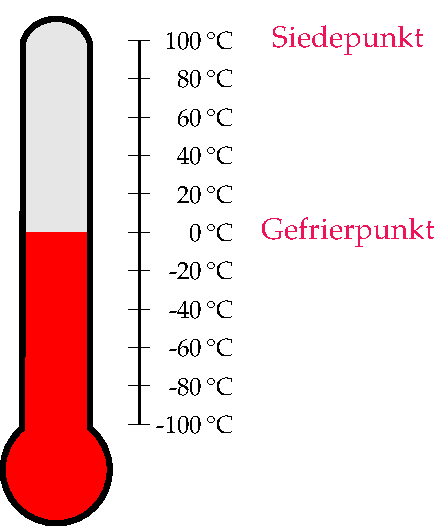
\includegraphics[width=\linewidth]{thermometer}
\end{wrapfigure}
Für viele Zwecke reichen die natürlichen Zahlen nicht aus.
Ist es heute z.B. \unit[30]{°C} warm und wir wollen es mit der Temperatur vor einem halben Jahr vergleichen, so stellen wir vielleicht fest, dass es heute \unit[35]{°C} wärmer ist als vor einem halben Jahr.
D.h. die Temperatur $x$ vor einem halben Jahr in \unit{°C} erfüllt die Gleichung:
\begin{align*}
	x + 35 = 30
\end{align*}
Diese Gleichung lässt sich nicht mit den natürlichen Zahlen lösen, wohl aber, wenn wir negative Zahlen zulassen.
Dann erhalten wir: $x = -5$\,, d.h. die Temperatur ist \unit[--5]{°C}\,.

\subsection{Weitere Beispiele}
Die folgenden Beispiele zeigen, dass im Alltag negative Zahlen oft in Verbindung mit einer künstlich festgelegten Null vorkommen.

\paragraph{Temperatur.}
In Europa misst man die Temperatur in \unit{°C}.
Diese Temperaturskala ist so definiert, dass bei Normaldruck der Gefrierpunkt des Wasser gleich \unit[0]{°C} entspricht und der Siedepunkt gleich \unit[100]{°C}.
Wenn eine Temperatur also unter der Temperatur des Wassergefrierpunkts ist, so ist sie negativ.

\paragraph{Meter über dem Meeresspiegel.}
Auf Landkarten wird die Höhe z.B. in Metern über dem Meeresspiegel (m ü.M.) angegeben.
Zum Beispiel liegt der Gipfel des Mt. Whitney in den USA \unit[4418]{m} über dem Meer, kurz \unit[4418]{m ü.M.}
Dabei wurde der Meeresspiegel künstlich als \emph{Normalhöhe} festgelegt.
Dies führt dazu, dass das sogenannte \emph{Tal des Todes} sich bei \unit[-86]{m ü.M.} befindet.

\subsection{Zahlengerade}
\begin{figure}[H]
	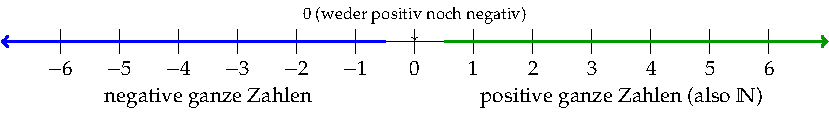
\includegraphics[width=\linewidth]{zahlengerade}
	\caption{Die Zahlengerade mit den positiven ganzen Zahlen rechts von der Null und den negativen ganzen Zahlen links von der Null.
	Die Null ist weder positiv noch negativ.}
	\label{fig:zahlengerade-pos-neg}
\end{figure}

Die sogenannten negativen ganzen Zahlen $-1, -2, -3, \ldots$ stehen links von 0 auf der Zahlengeraden, siehe Abbildung \ref{fig:zahlengerade-pos-neg}.
Die natürlichen Zahlen, die auch positive ganze Zahlen genannt werden, stehen rechts von Null auf der Zahlengeraden. Beachte, dass die Null selbst weder positiv noch negativ ist.
Möchtest du die Zahlen in $\N_0$ auf diese Weise bezeichnen (also die Null mit einschliessen), so kannst du sie nicht-negative ganze Zahlen nennen.

\section{Ganze Zahlen}
\begin{wrapfigure}{r}{7cm}
	\vspace{-1cm}
	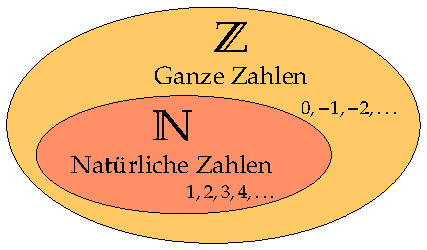
\includegraphics[width=\linewidth]{numberset-integers}
	% \caption{Die natürlichen Zahlen sind in den ganzen Zahlen enthalten.
	% Auf eine Darstellung der Menge $\N_0$ wurde hier für die bessere Übersicht verzichtet.}
	% \label{fig:numberset-integers}
	\vspace{-2cm}
\end{wrapfigure}
Die Menge der ganzen Zahlen besteht aus den natürlichen Zahlen, den negativen ganzen Zahlen und der Null.

Jede natürliche Zahl ist auch eine ganze Zahl, aber nicht andersherum.
D.h. die Menge der natürlichen Zahlen ist komplett in der Menge der ganzen Zahlen enthalten.
%, siehe Abbildung \ref{fig:numberset-integers}.

\vspace{1cm}
\begin{defn}{Ganzen Zahlen}
	Fügt man zu den natürlichen Zahlen $\N$ die Zahl 0 und die negativen ganzen Zahlen $-1, -2, -3,\ldots$ hinzu,
	so erhält man die Menge der ganzen Zahlen $\Z = \{ \ldots, -3, -2, -1, 0, 1, 2, 3, \ldots \}$\, .
\end{defn}


\subsection{Regeln}
Für das Rechnen mit den ganzen Zahlen gelten die arithmetischen Grundgesetze von Seite \pageref{law:arithmetic}, bis auf eine Ausnahme!
Welche? (Schreibe es selber auf.)\\
\kariert{15}{2}\\~\\
Vervollständige die Übersicht von Seite \pageref{law:arithmetic} für alle Regeln bis auf die, die nicht gilt:
\begin{law}{Arithmetische Grundgesetze für \underline{\bfseries die ganzen Zahlen}}
    \bgroup
    \def\arraystretch{2.5}
	\begin{tabularx}{\linewidth}{|X|p{3.7cm}|p{3.7cm}|}
			\hline
			 & Addition & Multiplikation \\
			\hline
			Kommutativgesetz &  &  \\\hline
			Assoziativgesetz &  &  \\\hline
			Es gibt Neutralelement\newline 0 bzw. 1\,. &  &  \\\hline
			Es gibt inverses Element\newline~ & & \\
			\hline
			Distributivgesetz & \multicolumn{2}{c|}{} \\
			\hline
    \end{tabularx}
    \egroup
\end{law}

\subsection{Subtraktion}
Mithilfe der negativen Zahlen kann man die Subtraktion als eine Addition mit einer negativen Zahl schreiben und so die Rechenregeln, die für die Addition gelten, anwenden, wie z.B. das Kommutativgesetz und das Assoziativgesetz.
\begin{example} Kommutativgesetz der Addition:
	\begin{align*}
					8 - 5		&\,=\, 8 + (-5) \,=\, (-5) + 8\\
		\text{Aber:}\quad 8 - 5		&\,\neq\, 5 - 8
	\end{align*}
	Wende das Kommutativgesetz einmal nach dem gleichen Schema selbst an:\\
	\kariert[\large 10 -- 3 \,=\,]{15}{1.5}\\
\end{example}
\begin{example} Assoziativgesetz der Addition:
	\begin{align*}
					(8 - 5) - 1			&\,=\, \bigl(8 + (-5)\bigr) + (-1) \,=\, 8 + \bigl( (-5) + (-1)\bigr)\\
		\text{Aber:}\quad (8 - 5) - 1	&\,\neq\, 8 - (5 - 1)
	\end{align*}
	Wende das Assoziativgesetz einmal nach dem gleichen Schema selbst an:\\
	\kariert[\large (10 -- 3) -- 2 \,=\,]{15}{2}\\
\end{example}
\begin{example} Minusklammer:
	\begin{align*}
					1 -(8 - 5)			&\,=\, 1 + (-1)\cdot\bigl(8 + (-5)\bigr)\,=\, 1 + (-1)\cdot 8 + (-1)\cdot (-5) = 1 - 8 + 5\\
	\end{align*}
	Wende die Minusklammer einmal nach dem gleichen Schema selbst an:\\
	\kariert[\large 10 -- (3 -- 2) \,=\,]{15}{2}\\
\end{example}

\section{Rationale Zahlen}
\begin{wrapfigure}{r}[1cm]{7cm}
	\vspace{-2cm}
	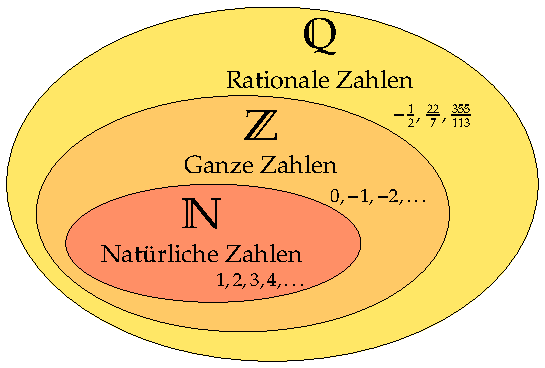
\includegraphics[width=\linewidth]{numberset-rational}
	\vspace{-2cm}
\end{wrapfigure}
In den arithmetischen Grundgesetzen für die ganzen Zahlen sehen wir, dass wir uns das inverse Element für die Multiplikation fehlt.
Führen wir dies ein, so erhalten wir die Menge der rationalen Zahlen $\Q$, die alle Zahlen enthält, die man als Bruch darstellen kann. 
\newpage
\begin{defn}{Rationale Zahlen}
	Die Menge der rationalen Zahlen $\Q$ besteht aus allen Zahlen, die man als Bruch schreiben kann.
	\begin{align*}
		\Q = \left\{\left. \frac{p}{q} ~\right|~ p,q \in \Z;~ q \neq 0\, \right\}
	\end{align*}
\end{defn}

~\\~\\
In dieser Menge können wir schon relativ viel machen.
Jedoch stellen wir fest, dass wir z.B. die Gleichung $x^2 = 2$ nicht über den rationalen Zahlen lösen können.

\begin{claim}
 Man kann $\sqrt{2}$ nicht als Bruch darstellen.
\end{claim}

\begin{proof}
 Schreibe hier den Beweis nochmal für dich selbst auf.
 \vfill
\end{proof}

\newpage
\subsection{Abbrechende und periodische Dezimalzahlen}
\label{sec:periodic}

~\vspace{.5cm}
\begin{law}{Brüche sind entweder abbrechende oder periodische Dezimalzahlen.}
\label{law:rationalsArePeriodic}
	In der Dezimaldarstellung ist eine rationale Zahl entweder ein abbrechende Dezimalzahl oder eine periodische.
\end{law}
~
\begin{example}~
	\begin{enumerate}[a)]
		\setlength\itemsep{0pt}
		\item $\frac{1}{50} = 0.02$
		\item $\frac{7}{40} = 0.175$
		\item $\frac{2}{3} = 0.\overline{6}$
		\item $\frac{1}{7} = 0.\overline{142857}$
	\end{enumerate}
\end{example}

Angenommen, eine Zahl ist in der Dezimaldarstellung eine abbrechende Dezimalzahl.
Begründe anhand eines Beispiels, warum es dann möglich ist, den Nenner in der Form 10 oder 100 oder 1000 oder 10\,000 \ldots darzustellen:\\~\\
\kariert{15}{4}\\

Begründe, warum es deshalb für eine abbrechende Dezimaldarstellung notwendig ist, dass der Nenner der Zahl keine Primteiler abweichend von 2 und 5 enthält:\\~\\
\kariert{15}{4}

\newpage
\begin{xmpl}
	Hier sind zwei Beispiele für periodische Dezimalzahlen. Berechne die Dezimaldarstellung mithilfe der schriftlichen Division:\\
 
	\kariertTop[$3~~~:~~~7~=$]{14.5}{8}\\~\\
	\kariertTop[$6~~~:~~~1~~~1~=$]{14.5}{6}\\
\end{xmpl}

Begründe in eigenen Worten, warum Brüche in der Dezimaldarstellung entweder abbrechen oder periodisch werden.\\
\kariert{14.5}{3}

Jetzt wissen wir, wie wir vom Bruch zum Dezimalbruch kommen.%
\footnote{\begin{minipage}[t]{.85\linewidth}
			Quelle: \url{https://www.kapiert.de/mathematik/klasse-5-6/dezimalbrueche/}\\\url{periodische-dezimalbrueche-und-anwendungsaufgaben/}\\
			\url{periodische-dezimalbrueche-in-brueche-umwandeln/}, abgerufen am 03.09.2024.
		\end{minipage}
		\hfill
		\begin{minipage}[t]{.1\linewidth}
			~\\\vspace{-.8cm}
			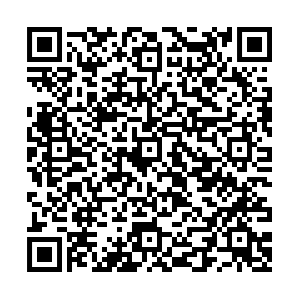
\includegraphics[width=\linewidth]{figures/QR-periodischeBrueche}
		\end{minipage}}
Aber schaffen wir es auch, aus einem periodischen Dezimalbruch den zugehörigen gewöhnlichen Bruch zu rekonstruieren?\\

Was ist z.B. $0.\overline{34}$ als Bruch geschrieben?
Teste selbst:\\
\kariertTop[$3~~~4~~~:~~~9~~~9~=$]{14.5}{4}\\
Warum funktioniert das?\\
Wir schreiben $0.\overline{34} \cdot 99$ auf folgende Weise:
\begin{align*}
	0.\overline{34} \cdot 99 &\,=\, 0.\overline{34} \cdot (100 - 1)
	\,=\, 0.\overline{34} \cdot 100 - 0.\overline{34} \cdot 1
	\,=\, 34.\overline{34} - 0.\overline{34}
	\,=\, 34\,.
\end{align*}
Versuche etwas ähnliches mit $0.\overline{567}$:\\
\kariert{14.5}{5}\\

Wandle auf einem Extrablatt noch die Zahlen $1.\overline{45}$ und $0.1\overline{56}$ in Brüche um.
Hefte dieses Blatt anschließend zu dieser Stelle im Skript.\\
Was du aus diesem Kapitel noch mitnehmen solltest, ist:

\begin{law}{Periodische Dezimalbrüche sind Brüche}
	\label{law:periodicIsRational}
	Ein periodischer Dezimalbruch lässt sich als Bruch aus zwei ganzen Zahlen darstellen.
\end{law}

\section{Reelle Zahlen}
\begin{wrapfigure}{r}[1cm]{8cm}
	\vspace{-1cm}
	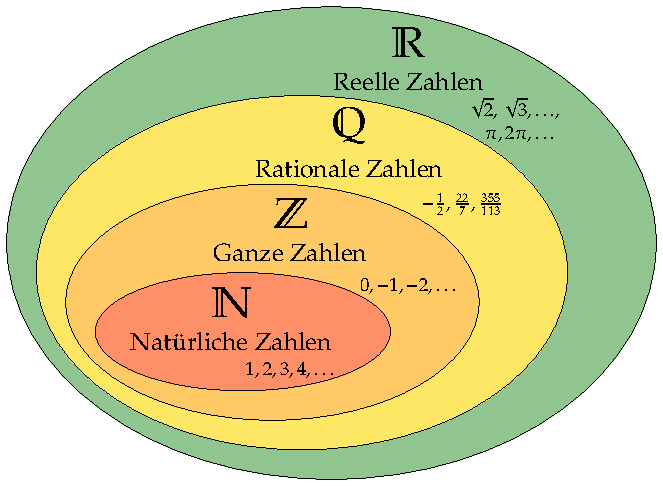
\includegraphics[width=\linewidth]{numberset-real}
	\vspace{-1cm}
\end{wrapfigure}
Da man $\sqrt{2}$ nicht als Bruch $\frac{p}{q}$ mit $p,q\in\Z$ darstellen kann, gilt:
\begin{align*}
  \sqrt{2} \notin \Q\, .
\end{align*}
Man nennt $\sqrt{2}$ eine sogenannte irrationale Zahl.
\begin{example}
 Kennst du bereits andere irrationale Zahlen? Welche?\\
 \kariert{7.5}{2}
\end{example}
\begin{example}
	Ist die Zahl rational oder irrational? Begründe.\\
	\begin{minipage}[t]{.3\linewidth}
		\begin{enumerate}[a)]
			\item $2.093903$
			\item $\frac{44}{45}$
		\end{enumerate}
	\end{minipage}
	\hfill
	\begin{minipage}[t]{.3\linewidth}
		\begin{enumerate}[a)]
		\setcounter{enumi}{2}
			\item $\sqrt{144}$
			\item $1.\overline{07}$
		\end{enumerate}
	\end{minipage}
	\hfill
	\begin{minipage}[t]{.3\linewidth}
		\begin{enumerate}[a)]
		\setcounter{enumi}{4}
			\item $1.090\,090\,009\,\ldots$
			\item $\sqrt{12}$
		\end{enumerate}
	\end{minipage}
	\vspace{.5cm}~\\
	{\bfseries Lösung:}
	\begin{enumerate}[a)]
        \setlength\itemsep{0pt}
        \item rational, da abbrechende Dezimalzahl und deshalb als Bruch darstellbar
        \item rational, da Bruch
        \item rational, da $\sqrt{144} = 12$
        \item rational, da periodische Dezimalzahl, siehe auch den Kasten auf Seite \pageref{law:periodicIsRational}.
        \item irrational, da weder abbrechende noch periodische Dezimalzahl
        \item irrational, da $\sqrt{12} = 2\cdot\sqrt{3}$\,.\\
        Angenommen, ~$2\cdot \sqrt{3}$ wäre doch rational. Zeige, dass daraus folgen würde, dass $\sqrt{3}$ rational ist.\\~\\
        \kariert{14}{3}\\~\\
        Dies ist ein Widerspruch dazu, dass $\sqrt{3}$ irrational ist.\\
        Also ist $\sqrt{12} = 2\cdot \sqrt{3}$ irrational.
    \end{enumerate}
\end{example}

Zusammenfassend können wir folgende Regeln festhalten:

\begin{law}{Regeln zum Erkennen von rationalen und irrationalen Zahlen}
	Ist eine Zahl z.B. eine
	\begin{itemize}\setlength\itemsep{0pt}
		\item abbrechende Dezimalzahl oder
		\item ein Bruch aus zwei ganzen Zahlen oder
		\item die Wurzel aus einer Quadratzahl oder
		\item eine periodische Dezimalzahl,
	\end{itemize}
	{\bfseries so ist sie eine rationale Zahl.}\\
	Ist sie hingegen
    \begin{itemize}\setlength\itemsep{0pt}
		\item eine Dezimalzahl, die weder abbricht, noch periodisch wird oder
		\item die Wurzel aus einer natürlichen Zahl, die keine Quadratzahl ist,
	\end{itemize}
	{\bfseries so ist sie eine irrationale Zahl.}\\
\end{law}~\\

Zuammen bilden die Menge der rationalen Zahlen $\Q$ und die Menge der irrationalen Zahlen die Menge der sogenannten reellen Zahlen $\mathbb{R}$.
In dieser Menge, bzw. diesem Zahlenbereich gelten alle arithmetischen Rechengesetze von \pageref{law:arithmetic}.\\

\begin{defn}{Reelle Zahlen}
	Die Menge der reellen Zahlen $\R$ besteht aus allen rationalen und allen irrationen Zahlen.
	Es handelt sich um die Menge aller möglichen Zahlen, die man auf der Zahlengeraden darstellen kann.
\end{defn}

\newpage
\subsection{Die Zahlengerade}
Erkläre anhand einer Zeichnung, wir man die Wurzel aus 2 auf der Zahlengerade darstellen kann:\\~\\
 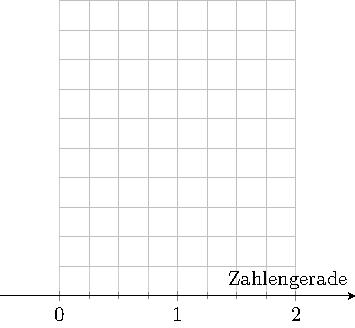
\includegraphics[width=.6\linewidth]{zahlengerade-Wurzel2}\\
\vspace{7cm}



\subsection{Für Interessierte: Gibt es Zahlen, die nicht reell sind?}
Bisher wurden die Erweiterungen der Zahlenbereiche dadurch begründet, dass uns (d.h. der Menschheit) der jeweils alte Zahlenbereich nicht ausgereicht hat, um bestimmte Gleichungen zu lösen.
Zum Beispiel konnten wir im Zahlenbereich der natürlichen Zahlen $\N$ die Gleichung $3 + x = 1$ nicht lösen.
Also haben wir die ganzen Zahlen $\Z$ eingeführt und konnten die Gleichung nun durch $x = -2$ lösen.

Dann hat uns z.B. die Lösung der Gleichung $3\cdot x = 1$ gefehlt -- also haben wir die rationalen Zahlen eingeführt und konnten nun $x = \frac{1}{3}$ setzen.
Als nächsten wollten wir die Gleichung $x^2 = 2$ lösen und haben festgestellt, dass uns hierzu wiederum die rationalen Zahlen nicht ausreichen.
Also haben wir unseren Zahlenbereich auf den Bereich der reellen Zahlen $\R$ erweitert und erhielten so die irrationale Zahl $\sqrt{2}$ als Lösung.
Hier waren wir aber nicht ganz konsequent, denn die Gleichung
\begin{align*}
	x^2 = -1
\end{align*}
können wir immer noch nicht lösen.
Egal, welche reelle Zahl wir für $x$ einsetzen, das Ergebnis von $x^2$ wird immer nicht nicht-negativ sein.

Um die obige Gleichung zu lösen, wurde ein neuer Zahlenbereich eingeführt -- der Zahlenbereich der komplexen Zahlen $\C$.
Dieser enthält u.a. die sogenannte \emph{imaginäre Einheit $\im$}, die genau so definiert ist, dass
\begin{align*}
	\im^2 = -1
\end{align*}
gilt.
Die Vielfachen von $\im$, wie z.B. $2\im, 3\im\, 4\im, \ldots$ nennen wir \emph{imaginäre Zahlen} und die Kombinationen $x + \im y$ mit $x$ und $y$ aus $\R$ nennen wir komplexe Zahlen, also z.B.:
\begin{align*}
	1 + \im \in \C;\qquad 2 - \im \in \C;\qquad 0.25 + 1.75\im \in \C \qquad \text{etc.}
\end{align*}

Zur grafischen Darstellung der komplexen Zahlen reicht uns die Zahlengerade nicht mehr aus.
Stattdessen verwenden wir die sogenannte \emph{komplexe Zahlenebene}, mit einem Koordinatensystem, dessen $x$-Achse die reellen Zahlen darstellt und dessen $y$-Achse die imaginären, siehe Abbildung \ref{fig:complexPlain}.
Die komplexe Zahl $1 + \im$ entspricht dann einem Punkt mit den Koordinaten $(1\,|\,1)$, die komplexe Zahl $2 - \im$ entspricht dem Punkt $(2\,|\,-1)$.
\begin{figure}[H]
	\centering
	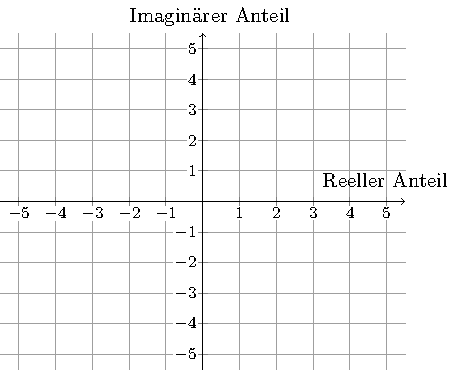
\includegraphics[width=.6\linewidth]{KomplexeEbene}
	\caption{Die komplexe Zahlenebene.}
	\label{fig:complexPlain}
\end{figure}



% \section{Kann man alle Zahlen als Bruch darstellen?}
% Hier muss noch etwas Geschichte hin.
